% !TeX root = RJwrapper.tex
\title{GCalignR. An R package for aligning Gas-Chromatography data}
\author{by Meinolf Ottensmann, Martin A. Stoffel, Joseph I. Hoffman}

\maketitle

\abstract{%
Chemical signals are among the most fundamental and oldest means of
animal communication. The desire to unravel broader patterns of chemical
communication in birds and mammals paved the way for two not entirely
new techniques, gas-chromatography and mass-spectrometry, in the fields
of ecology and evolution. Comparing chemical profiles or chromatograms
across many individuals yields some major obstacles as even the newest
GC machines have an inherent error when measuring the retention times of
chemical substances. Here we present GCalignR, an R package for the
alignment of chromatography peaks among samples prior to hypothesis
testing using multivariate statistics. GCalignR is specifically designed
to be used by non-chemists by providing easy to use functions to check
and align gas-chromatography data based on retention times. In addition,
the package implements heatmaps and other plots to evaluate and
potentially adjust the peak alignment. We hope that GCalignR will
provide a tool that fits into a common biologist's workflow in R and
that the package will contribute to the standardization and
reproducibility of studies on chemical communication.
}

\subsection{Introduction}\label{introduction}

Chemical cues are arguably the most common mode of communication among
animals \citep{Wyatt.2014}. Patterns in complex chemical signatures can
therefore yield information about phylogenetic relatedness
\citep{Meulemeester.2011}, sexual maturation \citep{Caspers.2011},
kinship \citep{Bonadonna.2012, Krause.2012, Stoffel.2015} and genetic
quality \citep{Charpentier.2010, Leclaire.2012, Stoffel.2015}. One of
the most common approaches for resolving the chemical composition of
samples is gas-chromatography (GC), which can rapidly detect and
quantify molecules within a sample to generate a characteristic
chromatogram or chemical profile \citep{McNair.2011}. Although GC is
relatively rapid and inexpensive, making it attractive for studies of
non-model organisms, individual molecules are characterised according to
their retention times, making them effectively anonymous. An additional
mass-spectrometry step (GC-MS) can provide further details of the
chemical composition of individual molecules, allowing them to be
compared to existing databases where available. \par
GC provides a fast and effective means of resolving broad patterns of
chemical similarity, but relies heavily on the correct alignment of
homologous substances, represented by specific peaks, across samples.
However, peak alignment is not necessarily straightforward as it is
necessary to account for perturbations in retention times caused by
subtle, random and often unavoidable experimental variation including
changes in ambient temperature, flow rate of the carrier gas and column
ageing \citep{Scott.2003, Pierce.2005}. Variation in peak intensities
both within and among samples can also contribute towards errors in
characterising chemical profiles. \par
GC is widely used in behavioural and ecological studies of (usually) non
model organisms, such as birds, mammals and insects, where the goal is
often to investigate broad chemical patterns. These studies tend to use
GC-MS less often than studies of humans and other model organisms, both
because GC-MS is relatively expensive and because many of the chemicals
that are resolved often reveal limited homology to currently available
databases. However, aligning GC data is non-trivial due to the anonymous
nature of the many peaks. Consequently, although a number of programs
are available for aligning GC-MS data, which make use mass spectrograms,
we are only aware of a single program that can handle GC data
\citep{Dellicour.2013}. As a result, most studies of mammalian and avian
chemical communication have relied on manual alignment and peak calling
\citep{Drea.2013}, which is time-consuming, particularly for large
samples of individuals, can be biased and subjective, and is not
strictly reproducible. \par
Here, we introduce GCalignR, an R package that implements a simple
algorithm to align peaks based on retention time data obtained by GC and
provides sophisticated visualisations for the evaluation of alignment
quality. First of all, the \texttt{check\_input} function is used to
ensure that the data are formatted correctly (figure
\href{figure:workflow}, (1)). Second, the \texttt{align\_chromatograms}
function is used to align the data (figure \href{figure:workflow} (2))
as follows: (i) systematic shifts of chromatograms are corrected by
applying appropriate linear shifts to whole chromatograms based on a
single reference sample; (ii) retention times of individual peaks are
grouped iteratively together with homologous peaks of other samples and
aligned within the same row in a retention time matrix; and (iii) rows
with similar retention times are merged where appropriate. Third,
diagnostic plots allow the resulting alignments to be visually inspected
(figure \href{figure:workflow} (3)), thereby facilitating optional
pre-processing or re-alignment of the data (figure
\href{figure:workflow} (4)). Finally, to compensate for differences in
total chemical concentrations among samples, measures of peak abundance
(e.g.~peak area or peak height) can be normalised using the function
norm\_peaks (figure \href{figure:workflow} (5)). \par
Implementing GC alignment and checking within R brings several
advantages over currently available stand-alone programs. First, the
code is open source, which facilitates flexibility and transparency in
data analysis. Second, all computational steps can be integrated into R
Markdown documents \citep{Allaire.2016}, thereby enhancing
reproducibility. Finally, our package provides a seamless transition
from the processing of the peak data through to downstream analysis
within other widely used R packages for multivariate analysis, e.g.
\href{https://CRAN.R-project.org/package=vegan}{\CRANpkg{vegan}}
\citep{Oksanen.2016}.

\subsection{The Package}\label{the-package}

GCalignR contains functions to align peaks from GC and GC-MS data based
on retention times and evaluate the resulting alignments. The main aim
of the package is to provide a simple tool that guides the user through
the alignment of large datasets prior to the statistical analysis of
multivariate chemical data. A typical workflow for the analysis of
chemical signatures in GCalignR is shown in figure \ref{figure:workflow}
and described below. The package vignette provides a detailed
description of all of the functions and their arguments and can be
accessed via \code{browseVignettes('GCalignR')} after the package has
been installed. The workflow is described below and the standard input
format of GCalignR is a tab-delimited text file, as illustrated in the
vignette.

\begin{figure}[htbp]
\centering
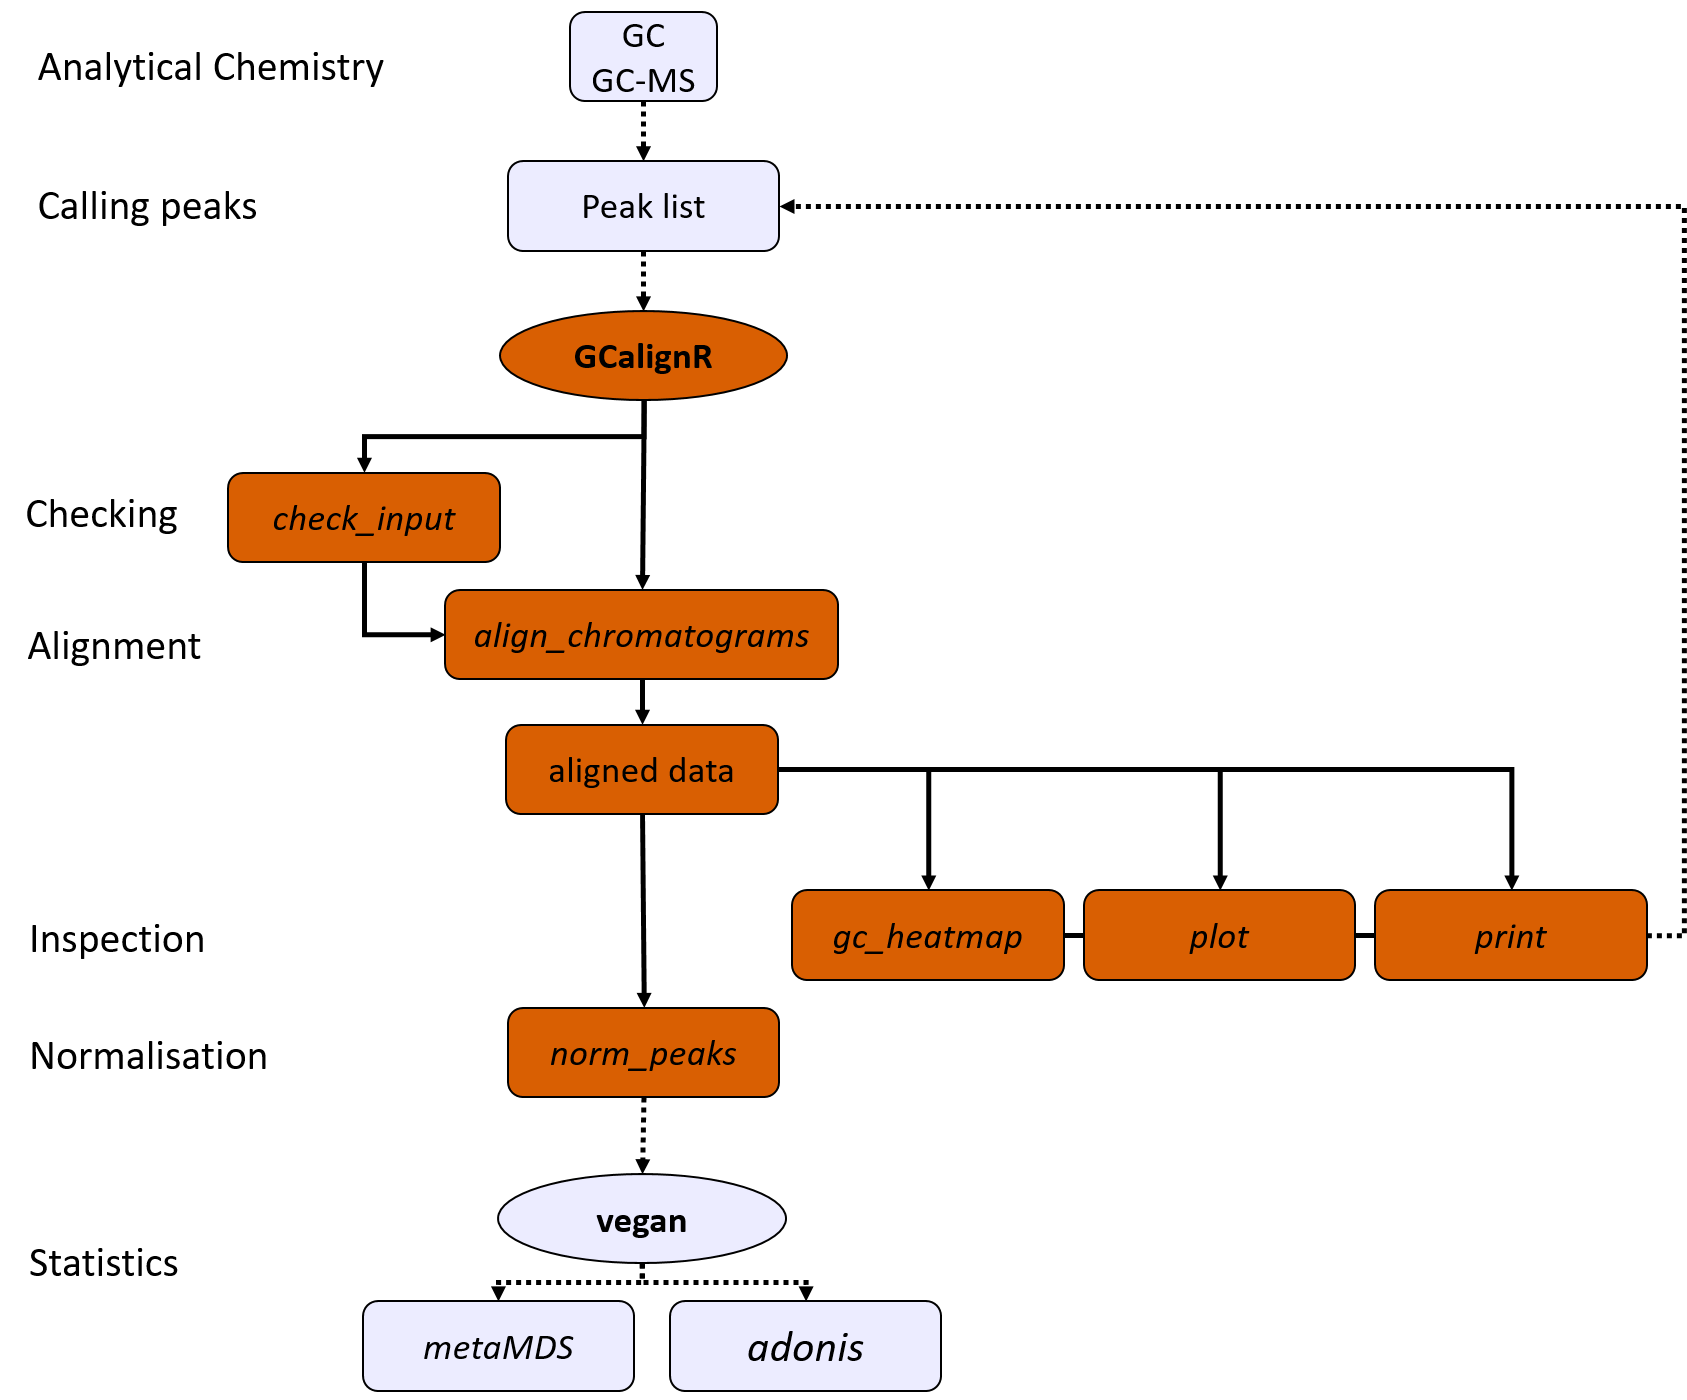
\includegraphics[width=13cm]{figures/workflow}
\caption{\pkg{GCalignR} workflow. In addition to the alignment of substances across samples, the package provides functions for checking and inspecting the data. The aligned data are ready to use for analyses in conjunction with other packages. Each function is explained within the main text.}
\label{figure:workflow}
\end{figure}

\subsubsection{Example dataset}\label{example-dataset}

The functionality of GCalignR is illustrated using GC data from skin
swabs of 41 Antarctic fur seal \emph{Arctocephalus gazella} mother-pup
pairs from two neighbouring breeding colonies at South Georgia in the
South Atlantic \citep{Stoffel.2015}. The chemical data associated with
these samples are provided in the file peak\_data.txt, which is
distributed with the package. Additional data on colony membership and
age-class are provided in the data frame peak\_factors.RData.

\subsection{Alignment of GC peaks among
samples}\label{alignment-of-gc-peaks-among-samples}

As outlined briefly above, the core algorithm in
\texttt{align\_chromatograms} (table \ref{table:parameter}) implements
three consecutive manipulations of the peak data (figure
\href{figure:workflow} i-iii) together with two further optional
manipulations (figure \href{figure:workflow} iv and v). These are
described in detail below.

\begin{table}[]
\centering
\caption{Important paramters altering the alignment of chemical datasets using the function align\_chromatograms}
\label{table:parameter}
\begin{tabular}{|p{5cm}|p{9cm}|} 
\textbf{Paramter} & \textbf{Description} \\ \midrule
blanks & Character vector containing the names of negative control samples (blanks) that are used to identify and remove contaminants \\
data & Path to a tab-delimited text file list containing the chemical data. See the vignette for an example and alternative input formats \\
del\_single\_peak & Logical that implements the optional functionality to remove unique substances from the aligned dataset \\
max\_diff\_peak2mean & Numeric value defining the allowed deviation of the retention time of a focal peak from the mean of the corresponding row during peak alignment \\
max\_linear\_shift & Numeric value (in minutes) that defines the range that is considered for the adjustment of linear shifts in peak retention times among samples \\
min\_diff\_peak2peak & Numeric values defining the expected minimum difference in retention times among substances. Rows that are more similar than the threshold value will be merged, if no conflict emerges due to the presence of peaks in more than one row within a single sample. \\
rt\_col\_name & Name of the variable containing retention times of peaks. The name needs to correspond to a variable included in the chemical data \\
reference & Name of a sample that will be used as reference to adjust linear shifts in peak retention times across samples. By default, a reference is automatically selected\\ \bottomrule
\end{tabular}
\end{table}\begin{figure}[htbp]
\centering
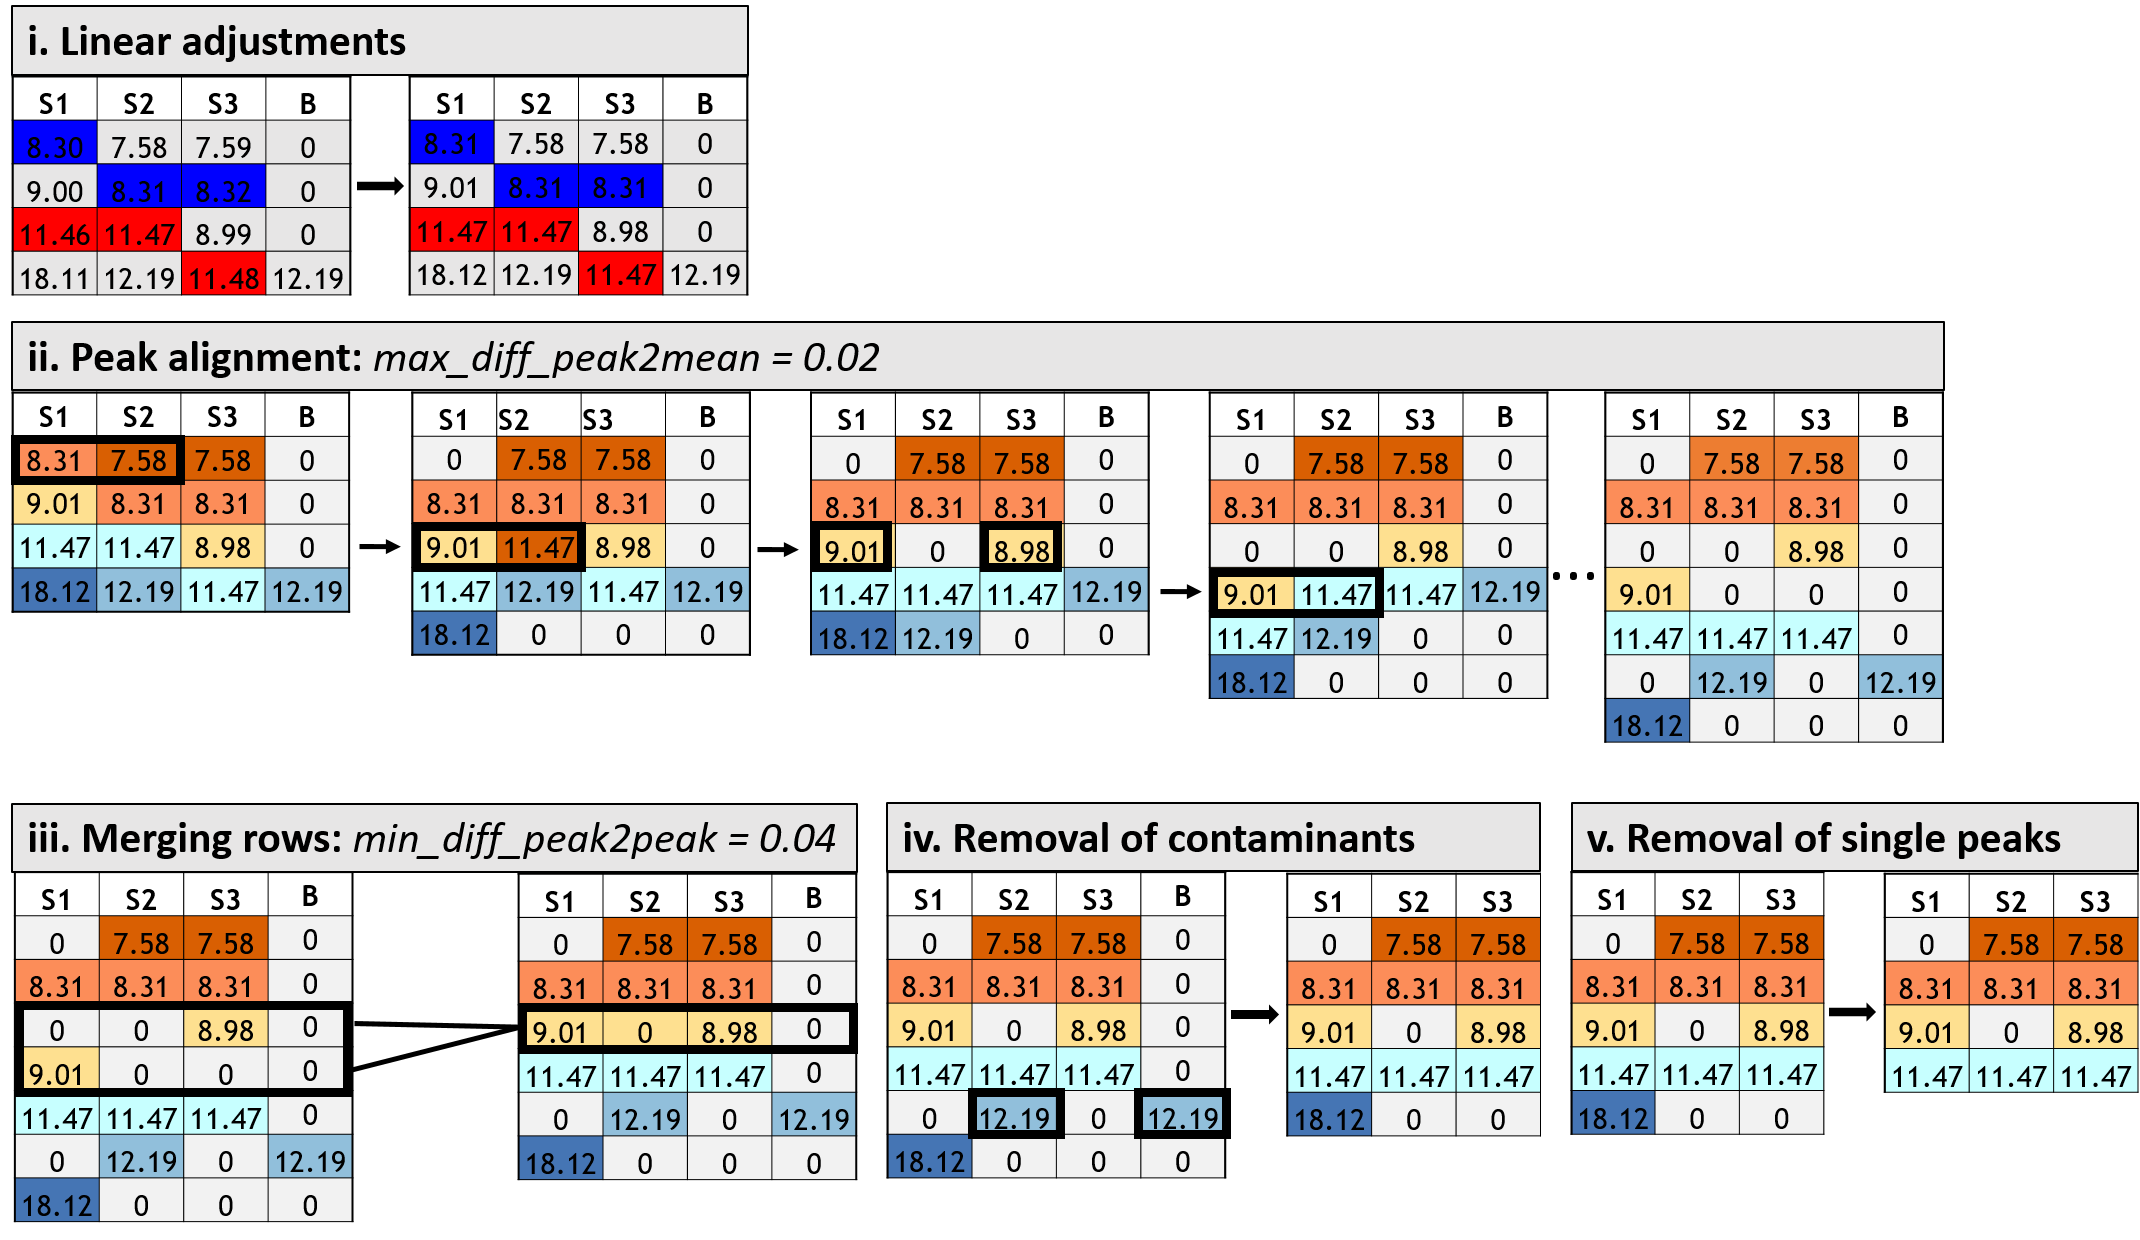
\includegraphics[width=13cm]{figures/algorithm_representation}
\caption{Overview of the alignment algorithm implemented in GCalignR uising a hypothetical dataste. Within each matrix, rows correspond to substances and columns correspond to samples. Consecutive manipulations of the matrices are shown from left to right. Zeros indicate absence of peaks and are therefore not considered in computations. \textbf{i}. Chromatograms are linearly shifted with respect to a reference (here S2). Linear adjustments in this example are conducted based on two peaks coloured in blue and red.  colouring of cells in \textbf{ii-v} refer to the substance identity in the final alignment and black rectangles indicate conflicts that cause manipulations. \textbf{ii}. Peaks are aligned row by row. Initially, always the second sample is compared to the first. Then the next sample is compared to all of the samples in previous columns until the last column is reached. \textbf{iii}. If merging does not result in the loss of any data, rows are merged. \textbf{iv}. If specified, all peaks found in one or more blanks (negative controls) are removed as well as the blank itself. \textbf{v}. Optionally, unique peaks present in a single sample are not of interest for similarity analyses and can be removed as well.}
\label{figure:algorithm}
\end{figure}

\subsubsection{(i) Linear adjustments of
chromatograms}\label{i-linear-adjustments-of-chromatograms}

First, all peaks within a chromatogram are shifted with respect to a
reference chromatogram to account for systematic shifts in retention
times among homologous chemicals shared among samples (figure
\href{figure:algorithm} i). This procedure is implemented for all of the
samples in such a way that the number of shared peaks is maximised. The
parameter \texttt{max\_linear\_shift} defines the maximum range of
linear shifts that are considered by the function. This approach clearly
relies on their being a sufficient number of substances shared among the
samples. In the absence of shared substances, the function will be
unlikely to find a suitable shift and consequently the chromatograms
will remain untransformed. By default, a reference is selected
automatically by searching for the sample with the highest average
similarity to all other samples based on the number of shared peaks
prior to alignment. Optionally, the alignment can be implemented using
an internal standard (labelled `reference') containing substances that
are known \emph{a priori} to occur in most or all of the samples.

\subsubsection{(ii) Peak alignment}\label{ii-peak-alignment}

Individual peaks are aligned across samples by comparing the peak
retention times of each sample consecutively with the mean of all
previous samples (figure \href{figure:algorithm} ii). If the focal cell
within the matrix contains a retention time that is larger than the mean
retention time of all previous cells within the same row plus a
user-defined threshold (equation \eqref{eq:one}), that cell is moved to
the next row.

\begin{equation}
\label{eq:one}
rt_{m} > \left(\frac{\sum_{i=1}^{m-1}rt_{i}}{m-1}\right) + max\textunderscore diff\textunderscore peak2mean
\end{equation}

where \texttt{rt} = retention time; \texttt{m} = focal cell and
\texttt{max\_diff\_peak2mean} defines the user-defined threshold
deviation from the mean retention time.

If the focal cell contains a retention time that is smaller than the
mean retention time of all previous cells within the same row minus a
user-defined threshold (equation \eqref{eq:two}), all previous retention
times are then moved to the next row.

\begin{equation}
\label{eq:two}
rt_{m} < \left(\frac{\sum_{i=1}^{m-1}rt_{i}}{m-1}\right) - max\textunderscore diff\textunderscore peak2mean
\end{equation}

After the last retention time of a row has been evaluated, this
procedure is repeated for the next row until the end of the retention
time matrix is reached.

\subsubsection{(iii) Merging rows}\label{iii-merging-rows}

Occasionally, due to minor variation in retention times, homologous
peaks can be sorted into different, but adjacent, rows in different
samples. However, this results in a clear pattern whereby some of the
samples will have a retention time in one of the rows while the other
samples will have a retention time in an adjacent row. Consequently, the
function merges adjacent rows when this does not cause any loss of
information (i.e.~no sample exists that contains substances in both
rows, (figure \href{figure:algorithm} iii). Again, the user can define
the threshold for the minimal difference in the retention time between
two mergeable peaks with \texttt{min\_diff\_peak2peak}. \par 

\subsubsection{(iv) Removal of
contaminants}\label{iv-removal-of-contaminants}

After aligning peaks, the package offers several optional
post-processing steps for cleaning up the data. First of all, negative
control samples, if available, can be used to remove potential
contaminants, including unwanted chemical substances in laboratory
reagents or within the gas chromatography column. Chemical data for
negative controls can be included in the input file and, by specifying
these samples as \texttt{blanks}, align\_chromatograms will remove all
substances present in the controls from the aligned dataset (figure
\href{figure:algorithm} iv).

\subsubsection{(v) Removal of single
peaks}\label{v-removal-of-single-peaks}

Frequently, substances occur only within a single sample. For
comparative approaches based on similarity matrices, these substances
are often not informative and can be removed from the dataset.
align\_chromatograms implements the removal of unique substances (figure
\href{figure:algorithm} v) when the \texttt{delete\_single\_peak}
argument is set to \texttt{TRUE}.

\subsection{Workflow}\label{workflow}

Here, we demonstrate a typical workflow in \texttt{GCalignR} using the
fur seal dataset as an example. All of the alignment steps described
above are implemented within the function \texttt{align\_chromatograms}.
A list of user-defined parameters and their descriptions can be accessed
from the documentation in the helpfile by typing
\texttt{?align\_chromatograms}. Prior to peak alignment, the
check\_input function interrogates the input file for typical formatting
errors and missing data. We encourage the use of unique names for
samples consisting only of letters, numbers and underscores. If the data
fail to pass this quality test, indicative warnings will be returned to
assist in error correction. As this function is executed internally
prior to any alignment, the data need to pass this check before the
alignment can begin.

\begin{Schunk}
\begin{Sinput}
library(GCalignR) # loads the package 
fpath <- system.file("extdata","peak_data.txt",package = "GCalignR") # path to peak_data.txt
check_input(fpath) # checks the data
\end{Sinput}
\begin{Soutput}
#> All checks passed!
\end{Soutput}
\end{Schunk}

In order to begin the alignment procedure, the following code needs to
be executed:

\begin{Schunk}
\begin{Sinput}
aligned_peak_data <- align_chromatograms(data = peak_data,
        rt_col_name = "time", # retention time variable
        max_diff_peak2mean = 0.02, # threshold for assigning peaks to rows
        min_diff_peak2peak = 0.08, # threshold for merging of rows
        max_linear_shift = 0.05, # threshold for linear adjustments
        delete_single_peak = TRUE, # removes unique peaks
        blanks = c("C2","C3")) # removes contaminants
\end{Sinput}
\end{Schunk}

Afterwards, a summary of the alignment process can be retrieved using
the printing method, which summarises the function call including
defaults that were not altered by the user. This provides all of the
relevant information to retrace every step of the alignment procedure.

\begin{Schunk}
\begin{Sinput}
print(aligned_peak_data) # verbal summary of the alignment procedure
\end{Sinput}
\begin{Soutput}
#> Summary of Peak Alignment running align_chromatograms
#> Input: peak_data
#> Start:  2017-02-01 18:04:11  Finished:  2017-02-01 18:41:11 
#> 
#> Call:
#>   GCalignR::align_chromatograms(data=peak_data, rt_col_name=time,
#>   max_linear_shift=0.05, blanks=(C2, C3), sep=\t, rt_cutoff_low=NULL,
#>   rt_cutoff_high=NULL, reference=NULL, max_diff_peak2mean=0.02,
#>   min_diff_peak2peak=0.08, delete_single_peak=FALSE)
#> 
#> Summary of scored substances:
#>    total   blanks retained 
#>      490      171      319 
#> 
#> In total 490 substances were identified among all samples. 171 substances were
#>   present in blanks. The corresponding peaks as well as the blanks were removed
#>   from the data. 319 substances are retained after all filtering steps.
#> 
#> Sample overview:
#>   The following 84 samples were aligned to the reference 'P31':
#>   M2, M3, M4, M5, M6, M7, M8, M9, M10, M12, M14, M15, M16, M17, M18, M19, M20,
#>   M21, M23, M24, M25, M26, M27, M28, M29, M30, M31, M33, M35, M36, M37, M38, M39,
#>   M40, M41, M43, M44, M45, M46, M47, M48, P2, P3, P4, P5, P6, P7, P8, P9, P10,
#>   P12, P14, P15, P16, P17, P18, P19, P20, P21, P23, P24, P25, P26, P27, P28, P29,
#>   P30, P31, P33, P35, P36, P37, P38, P39, P40, P41, P43, P44, P45, P46, P47, P48
#> 
#> For further details type...
#>   'gc_heatmap(aligned_peak_data)' to retrieve heatmaps
#>   'plot(aligned_peak_data)' to retrieve further diagnostic plots
\end{Soutput}
\end{Schunk}

As alignment quality may vary with the parameter values selected by the
user, the plot function can be used to output four diagnostic plots.
These allow the user to explore how the parameter values affect the
resulting alignment and can help flag issues with the raw data.

\begin{Schunk}
\begin{Sinput}
plot(aligned_peak_data) # diagnostic plots, can be envoke separately as well
\end{Sinput}
\end{Schunk}

\begin{figure}[htbp]
\centering
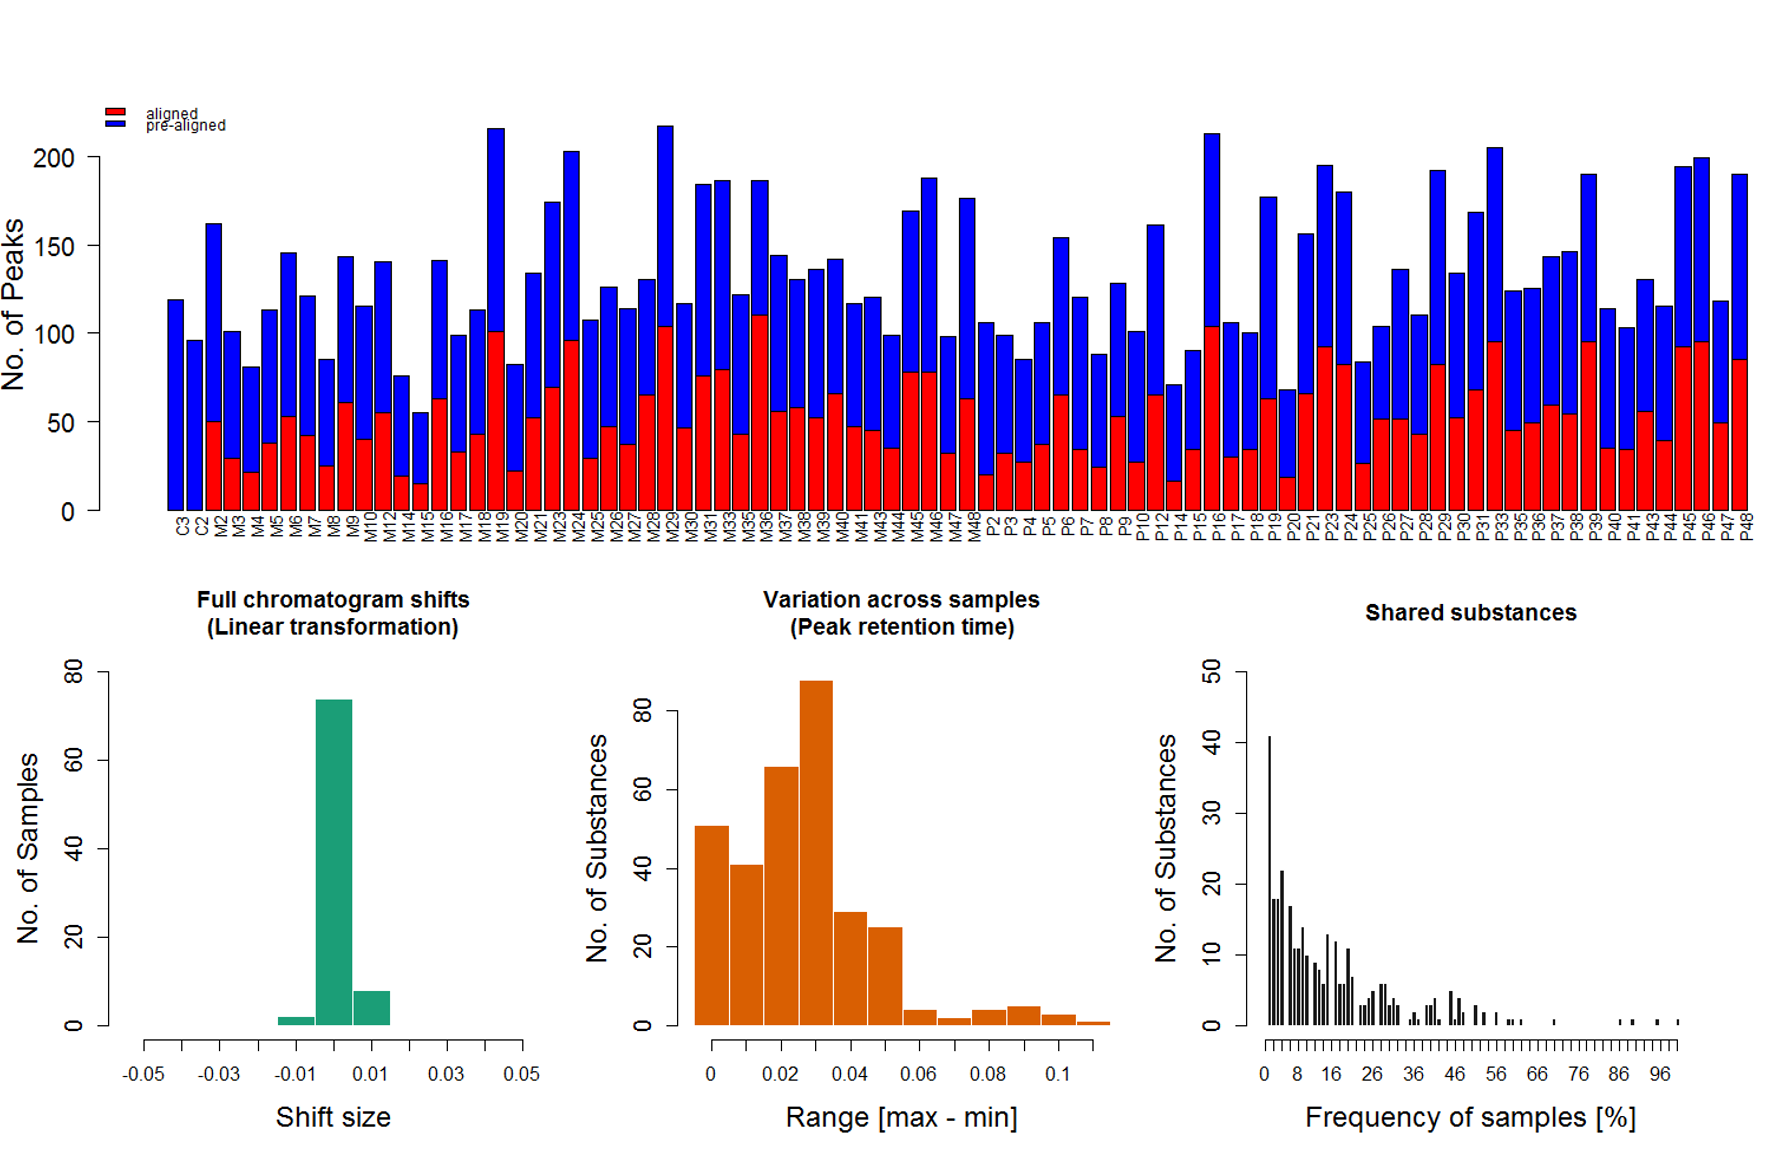
\includegraphics[width=15cm]{figures/plot_aligned_peak_data}
\caption{Diagnostic plots summarise aligned datasets.}
\label{figure:plot}
\end{figure}

Figure \href{figure:plot} a shows the distribution of peak numbers
across samples both before and after the alignment. In this example
dataset, we specified two negative controls (blanks): C2 and C3. After
the removal of substances shared with the controls as well as unique
substances, the number of post-alignment peaks is significantly reduced
across samples. For details of the number of removed substances, type
\texttt{print(aligned\_peak\_data)}. Figure \href{figure:plot} b shows a
histogram of linear shifts of entire samples implemented by the function
align\_chromatograms. The majority of samples were not shifted at all,
whereas a small number were shifted between -0.01 and 0.01 minutes.
\href{figure:plot} c shows a histogram of the amount of variation among
the samples in the retention times of single substances (defined as
retention times that were aligned based on user-defined criteria). In
this example, the distribution shows a left-skew, indicating that the
majority of substances vary less than 0.05 minutes. Finally, figure
\href{figure:plot} d shows the extent of sharing of substances across
samples. This shows a typical pattern whereby most of the substances are
found in a small number of samples but there a number of substances are
also present in most of the samples.

Additionally, the full alignment can be visualised using a heat map with
the function gc\_heatmap.

\begin{Schunk}
\begin{Sinput}
gc_heatmap(aligned_peak_data,type = "binary",threshold = 0.05)
\end{Sinput}
\end{Schunk}

\begin{figure}[htbp]
\centering
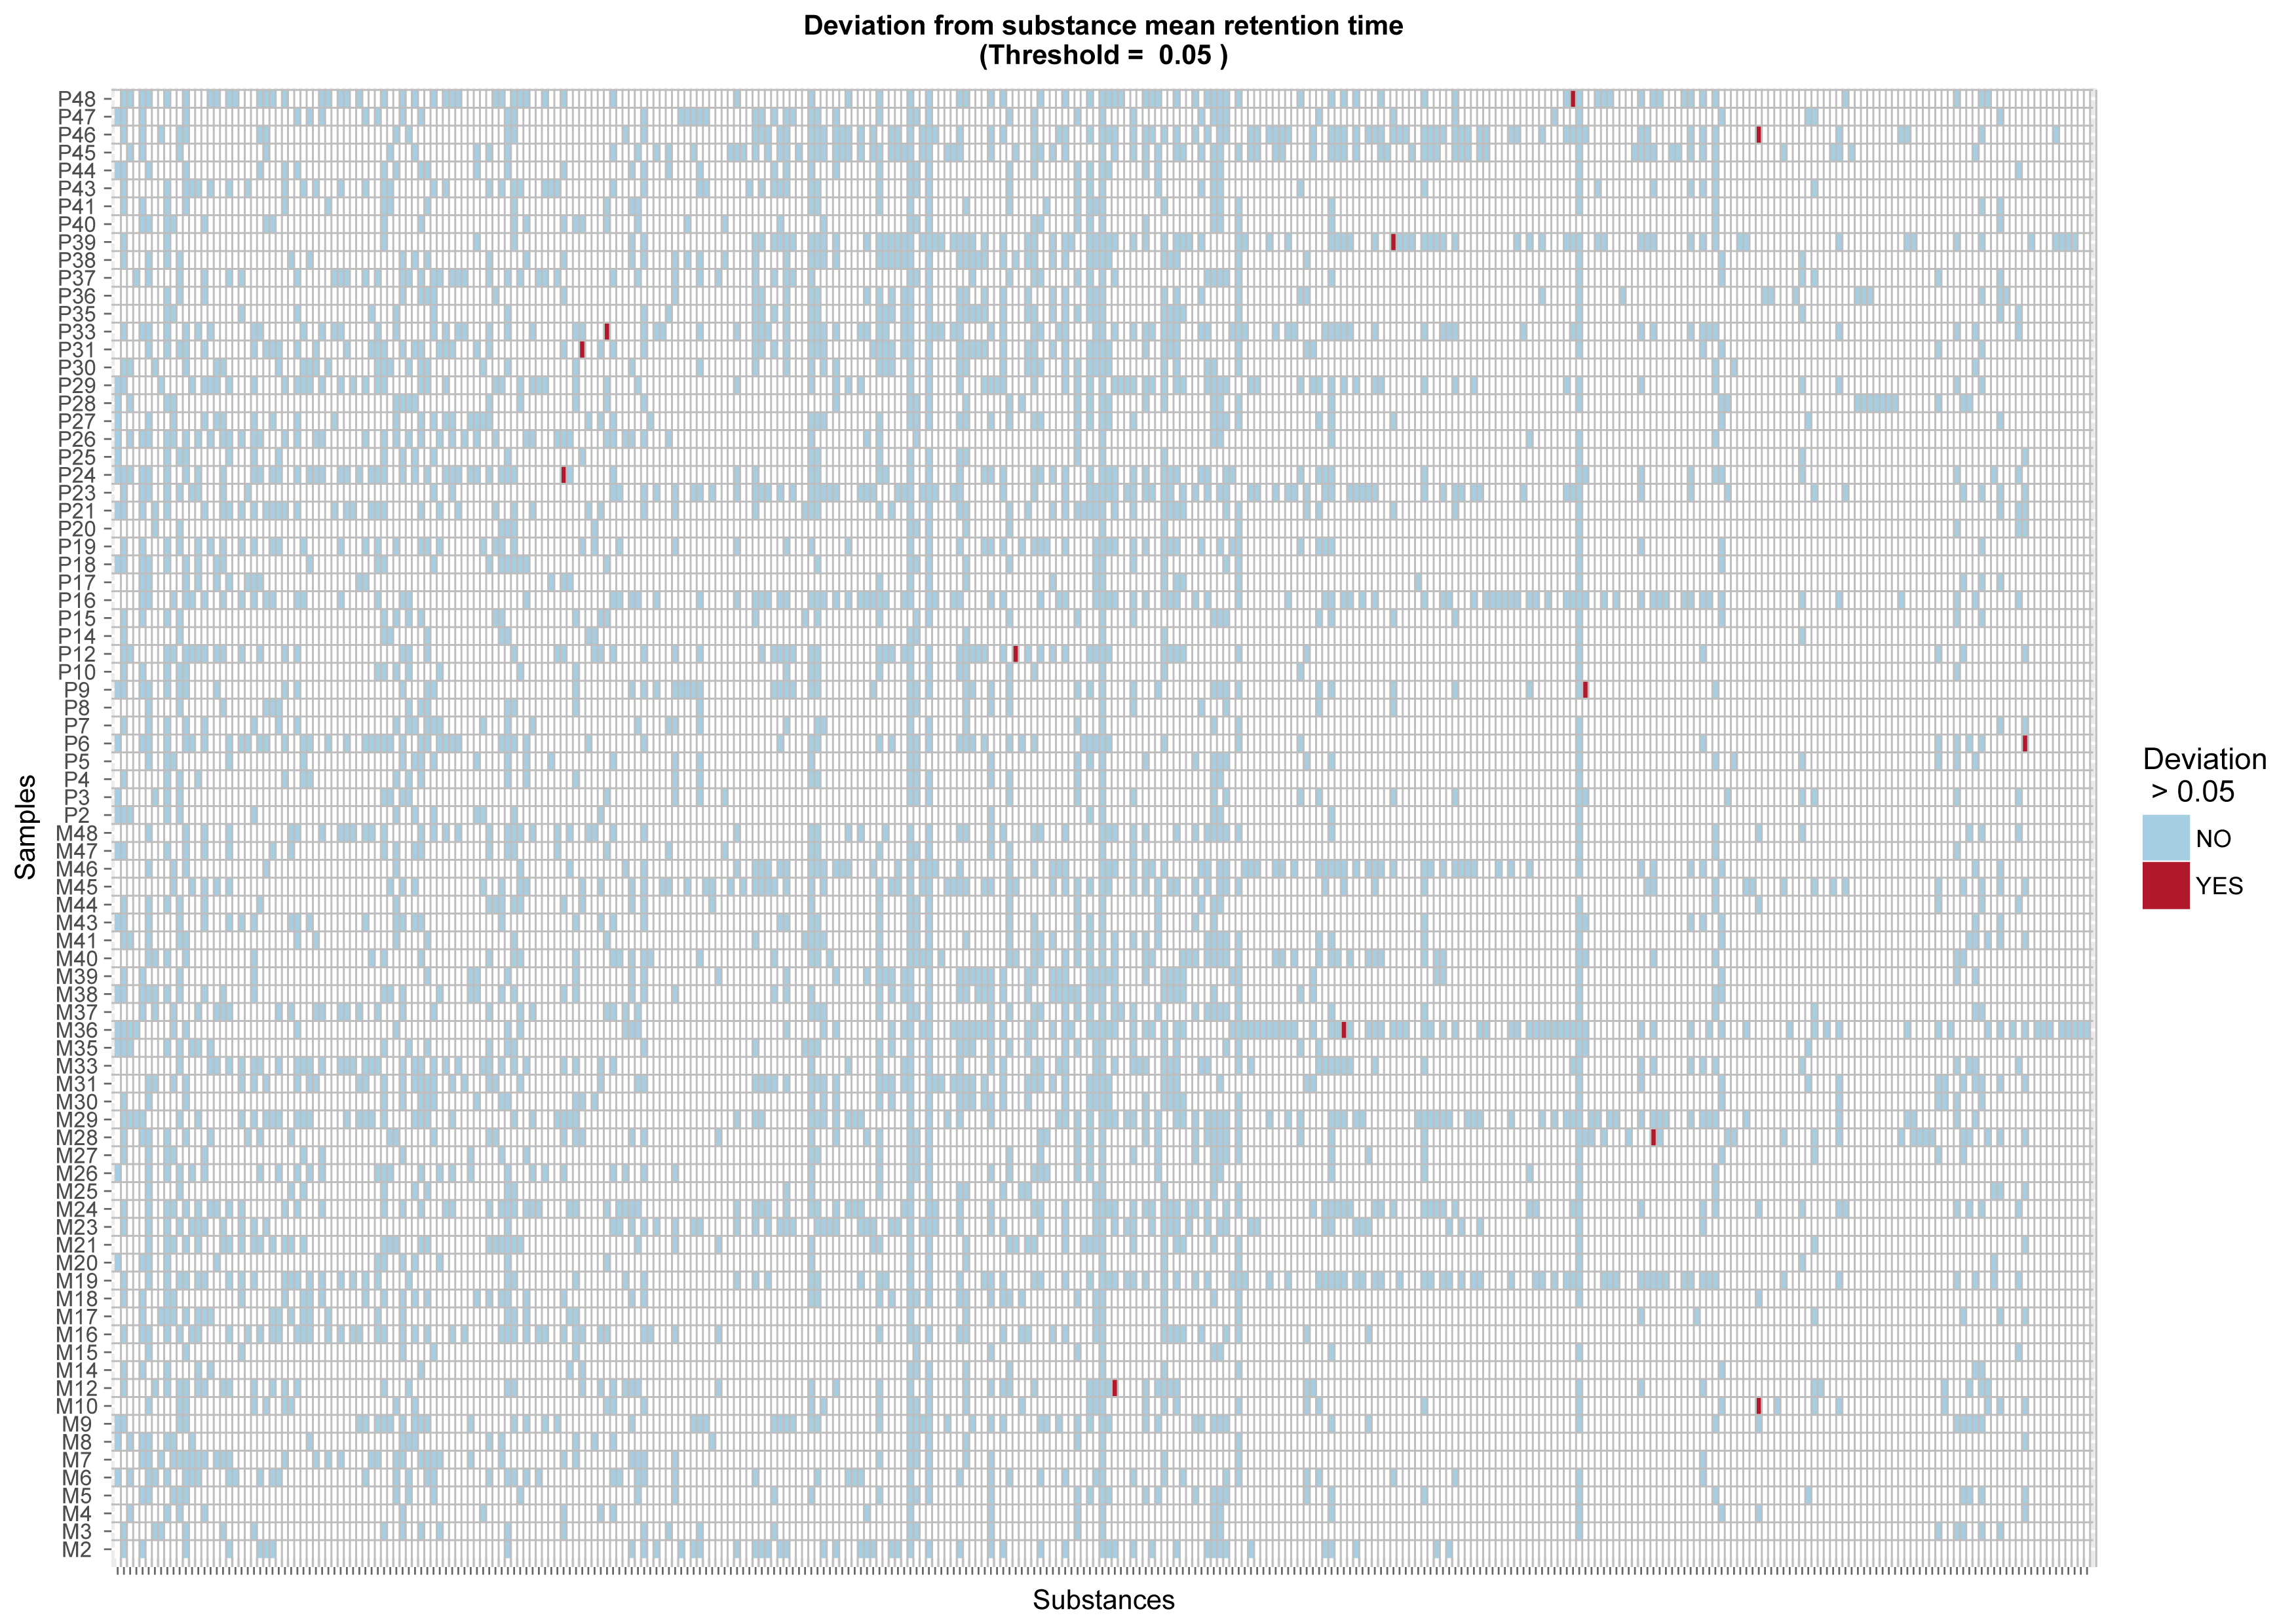
\includegraphics[width=13cm]{figures/heatmap}
\caption{Heatmaps allow to inspect the distribution of substances across samples as well as the variability of their retention times. Substances on the horizontal axis are ordered by retention times, increasing from left to right.}
\label{figure:heatmap}
\end{figure}

The resulting heatmap for the example dataset (figure
\href{figure:heatmap}) shows all of the post-alignment peaks across all
samples and substances. Filled cells represent peaks whereas empty cells
indicate the absence of a given substance within a sample. Substances
that deviate by less than a defined threshold value (in this case, 0.05
minutes) from the mean retention time across all samples are shown in
light blue. Red cells indicate a deviation that is larger than 0.05
minutes and thereby flag potentially problematic alignments. For the
example dataset, only a scattering of larger deviations are observed and
these do not appear to be clustered within samples or substances.

\subsubsection{Peak normalisation}\label{peak-normalisation}

In order to account for differences in the total concentration of
samples, we provide an additional function normalise\_peaks that can be
used to normalise peak abundances.

\begin{Schunk}
\begin{Sinput}
scent <- norm_peaks(data = aligned_peak_data,
                    rt_col_name = "time", # retention times
                    conc_col_name = "area", # peak area
                    out = "data.frame" ) # returns a data frame
\end{Sinput}
\end{Schunk}

\subsubsection{Downstream analyses}\label{downstream-analyses}

The output of GCalignR is compatible with other functionalities in R,
thereby providing a seamless transition between packages. For instance,
multivariate analyses can be conduced using the package \pkg{vegan}. To
visualise patterns of chemical similarity within the fur seal dataset in
relation to breeding colony membership, we implemented
non-metric-multidimensional scaling (NMDS) based on a Bray-Curtis
dissimilarity matrix and visualised the outcome using
\href{https://CRAN.R-project.org/package=ggplot2}{\CRANpkg{ggplot2}}
\citep{Wickham.2009}.

\begin{Schunk}
\begin{Sinput}
scent <- scent[match(row.names(peak_factors),row.names(scent)),] # sort data 
scent <- log(scent + 1) # log + 1 transformation
\end{Sinput}
\end{Schunk}

\begin{Schunk}
\begin{Sinput}
scent_nmds <- vegan::metaMDS(comm = scent,distance = "bray") # NMDS
scent_nmds <- as.data.frame(scent_nmds[["points"]]) # extract points
scent_nmds <- cbind(scent_nmds,colony = peak_factors[["colony"]]) # add factors
\end{Sinput}
\end{Schunk}

\begin{Schunk}
\begin{Sinput}
library(ggplot2) # load package ggplot2
ggplot(data = scent_nmds,aes(MDS1,MDS2,color = colony)) +
    geom_point(size = 2) + 
    theme_void() + 
    scale_color_manual(values = c("blue","red"), 
                       name="Breeding colony",
                       breaks=c("SSB", "FWB"),
                       labels=c("Special study beach", 
                                "Freshwater beach")) +
    theme(panel.background = element_rect(colour = "black", size = 1.5,fill = NA),aspect.ratio = 1,legend.justification=c(0,0), legend.position=c(0.01,0.01), legend.title = element_text(size=12, face="bold"),legend.background = element_rect(color = "black",fill = NA, size = 1, linetype = "solid")) 
\end{Sinput}
\end{Schunk}

\begin{figure}[htbp]
\centering
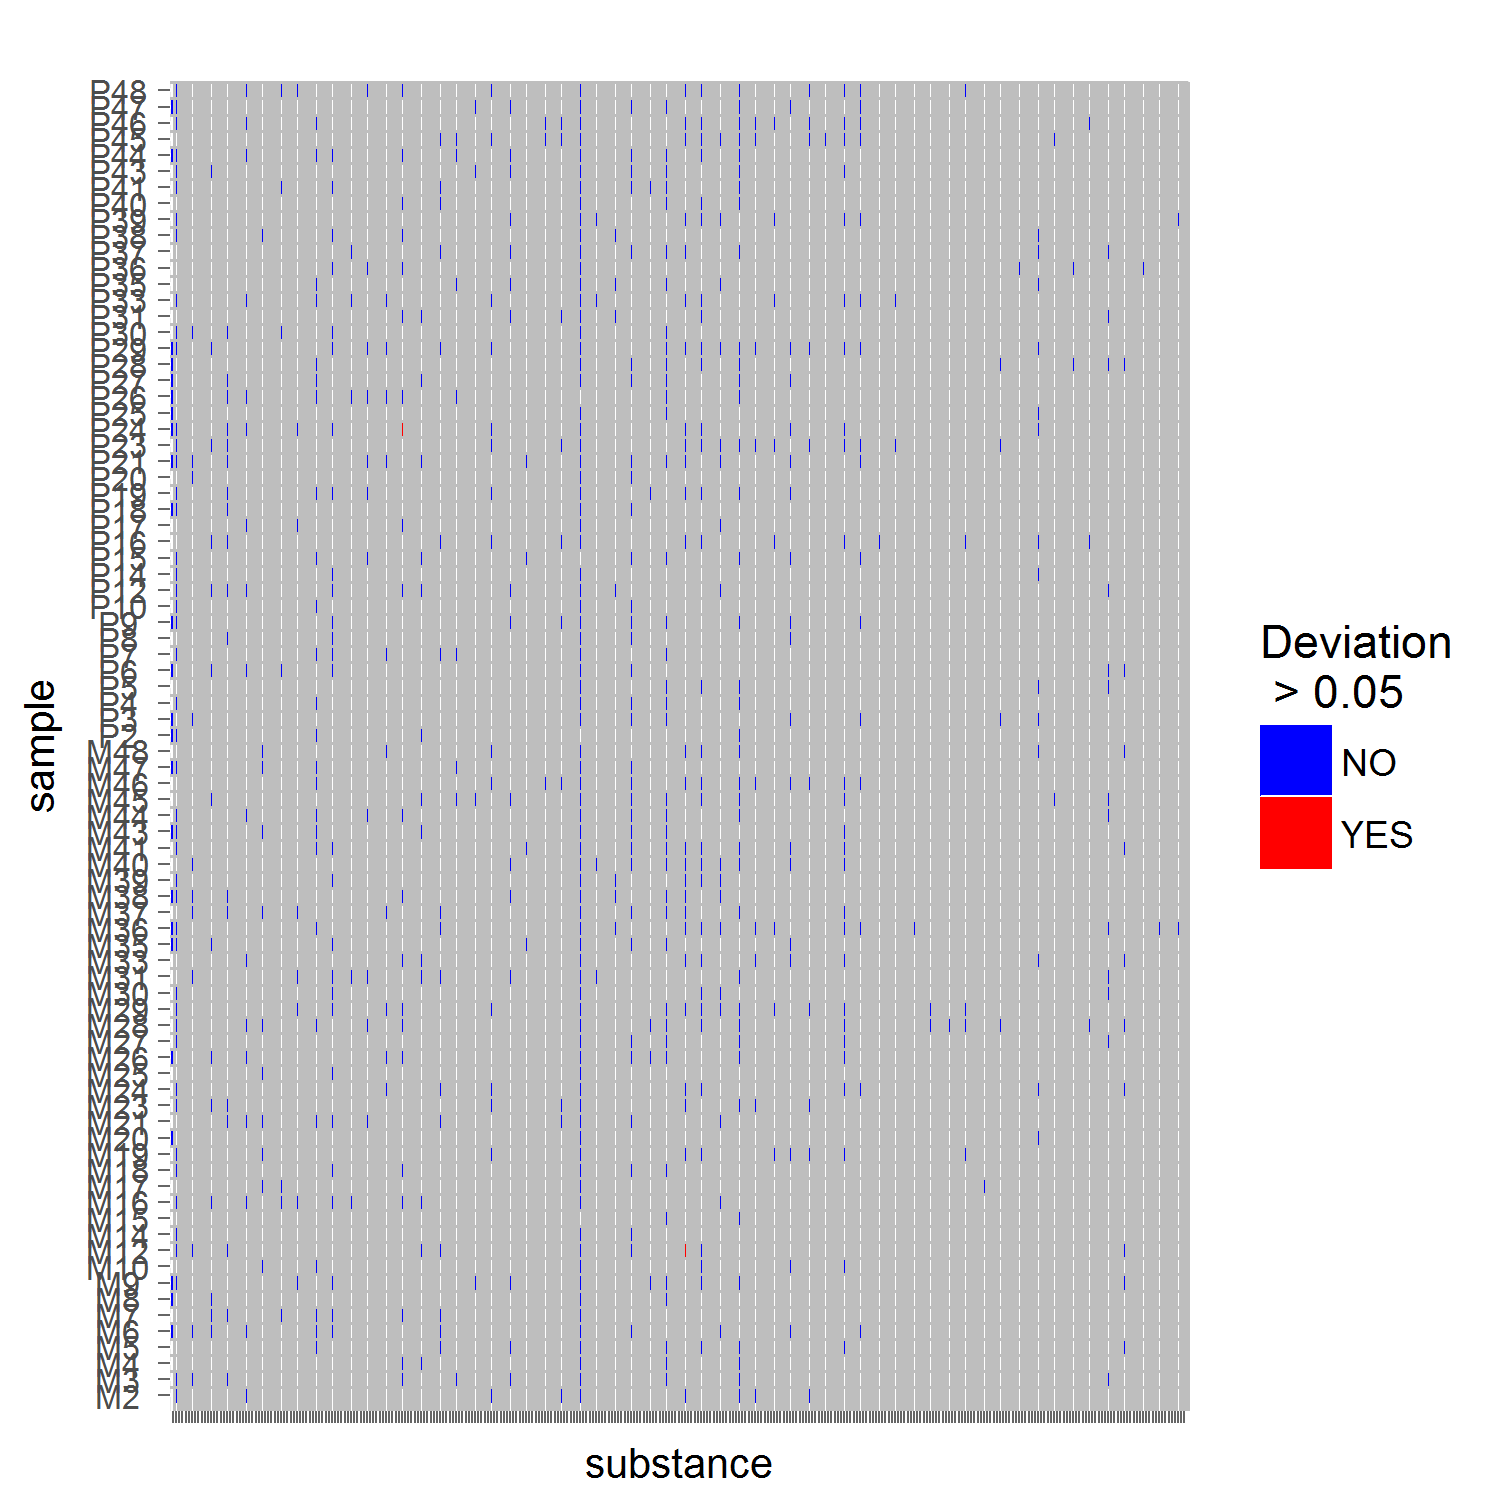
\includegraphics[width=13cm]{figures/ordiplot}
\caption{A NMDS plot shows the similarity of individuals within colonies. Ellipses indicate a confidence level of 0.95.}
\label{figure:ordiplot}
\end{figure}

Figure \href{figure:ordiplot} reveals a clear pattern in which seals
from the two colonies cluster separately based on their chemical
profiles, as shown also by \citet{Stoffel.2015}. Although a sufficient
number of standards were lacking to calculate the internal error rate
(as shown below for the bumblebee datasets), the strength of this
pattern, together with the rarity of substances invoking large
deviations from the mean retention time (figure \href{figure:heatmap}),
suggests that the alignment implemented by \texttt{GCalignR} is of high
quality. To explore this further, we introduced random errors into the
raw dataset, re-aligned the resulting datasets, and then quantified the
strength of clustering by colony using the function adonis from the
package vegan, which performs a permutation-based multivariate analysis
of variance (``permutational manova'', \citep{Anderson.2001}). The
introduced errors followed a Gaussian profile with -0.02 to 0.02. For
each error rate value, defined as the proportion of peaks within each
sample with random errors, we generated 10 datasets.

\begin{figure}[htbp]
\centering
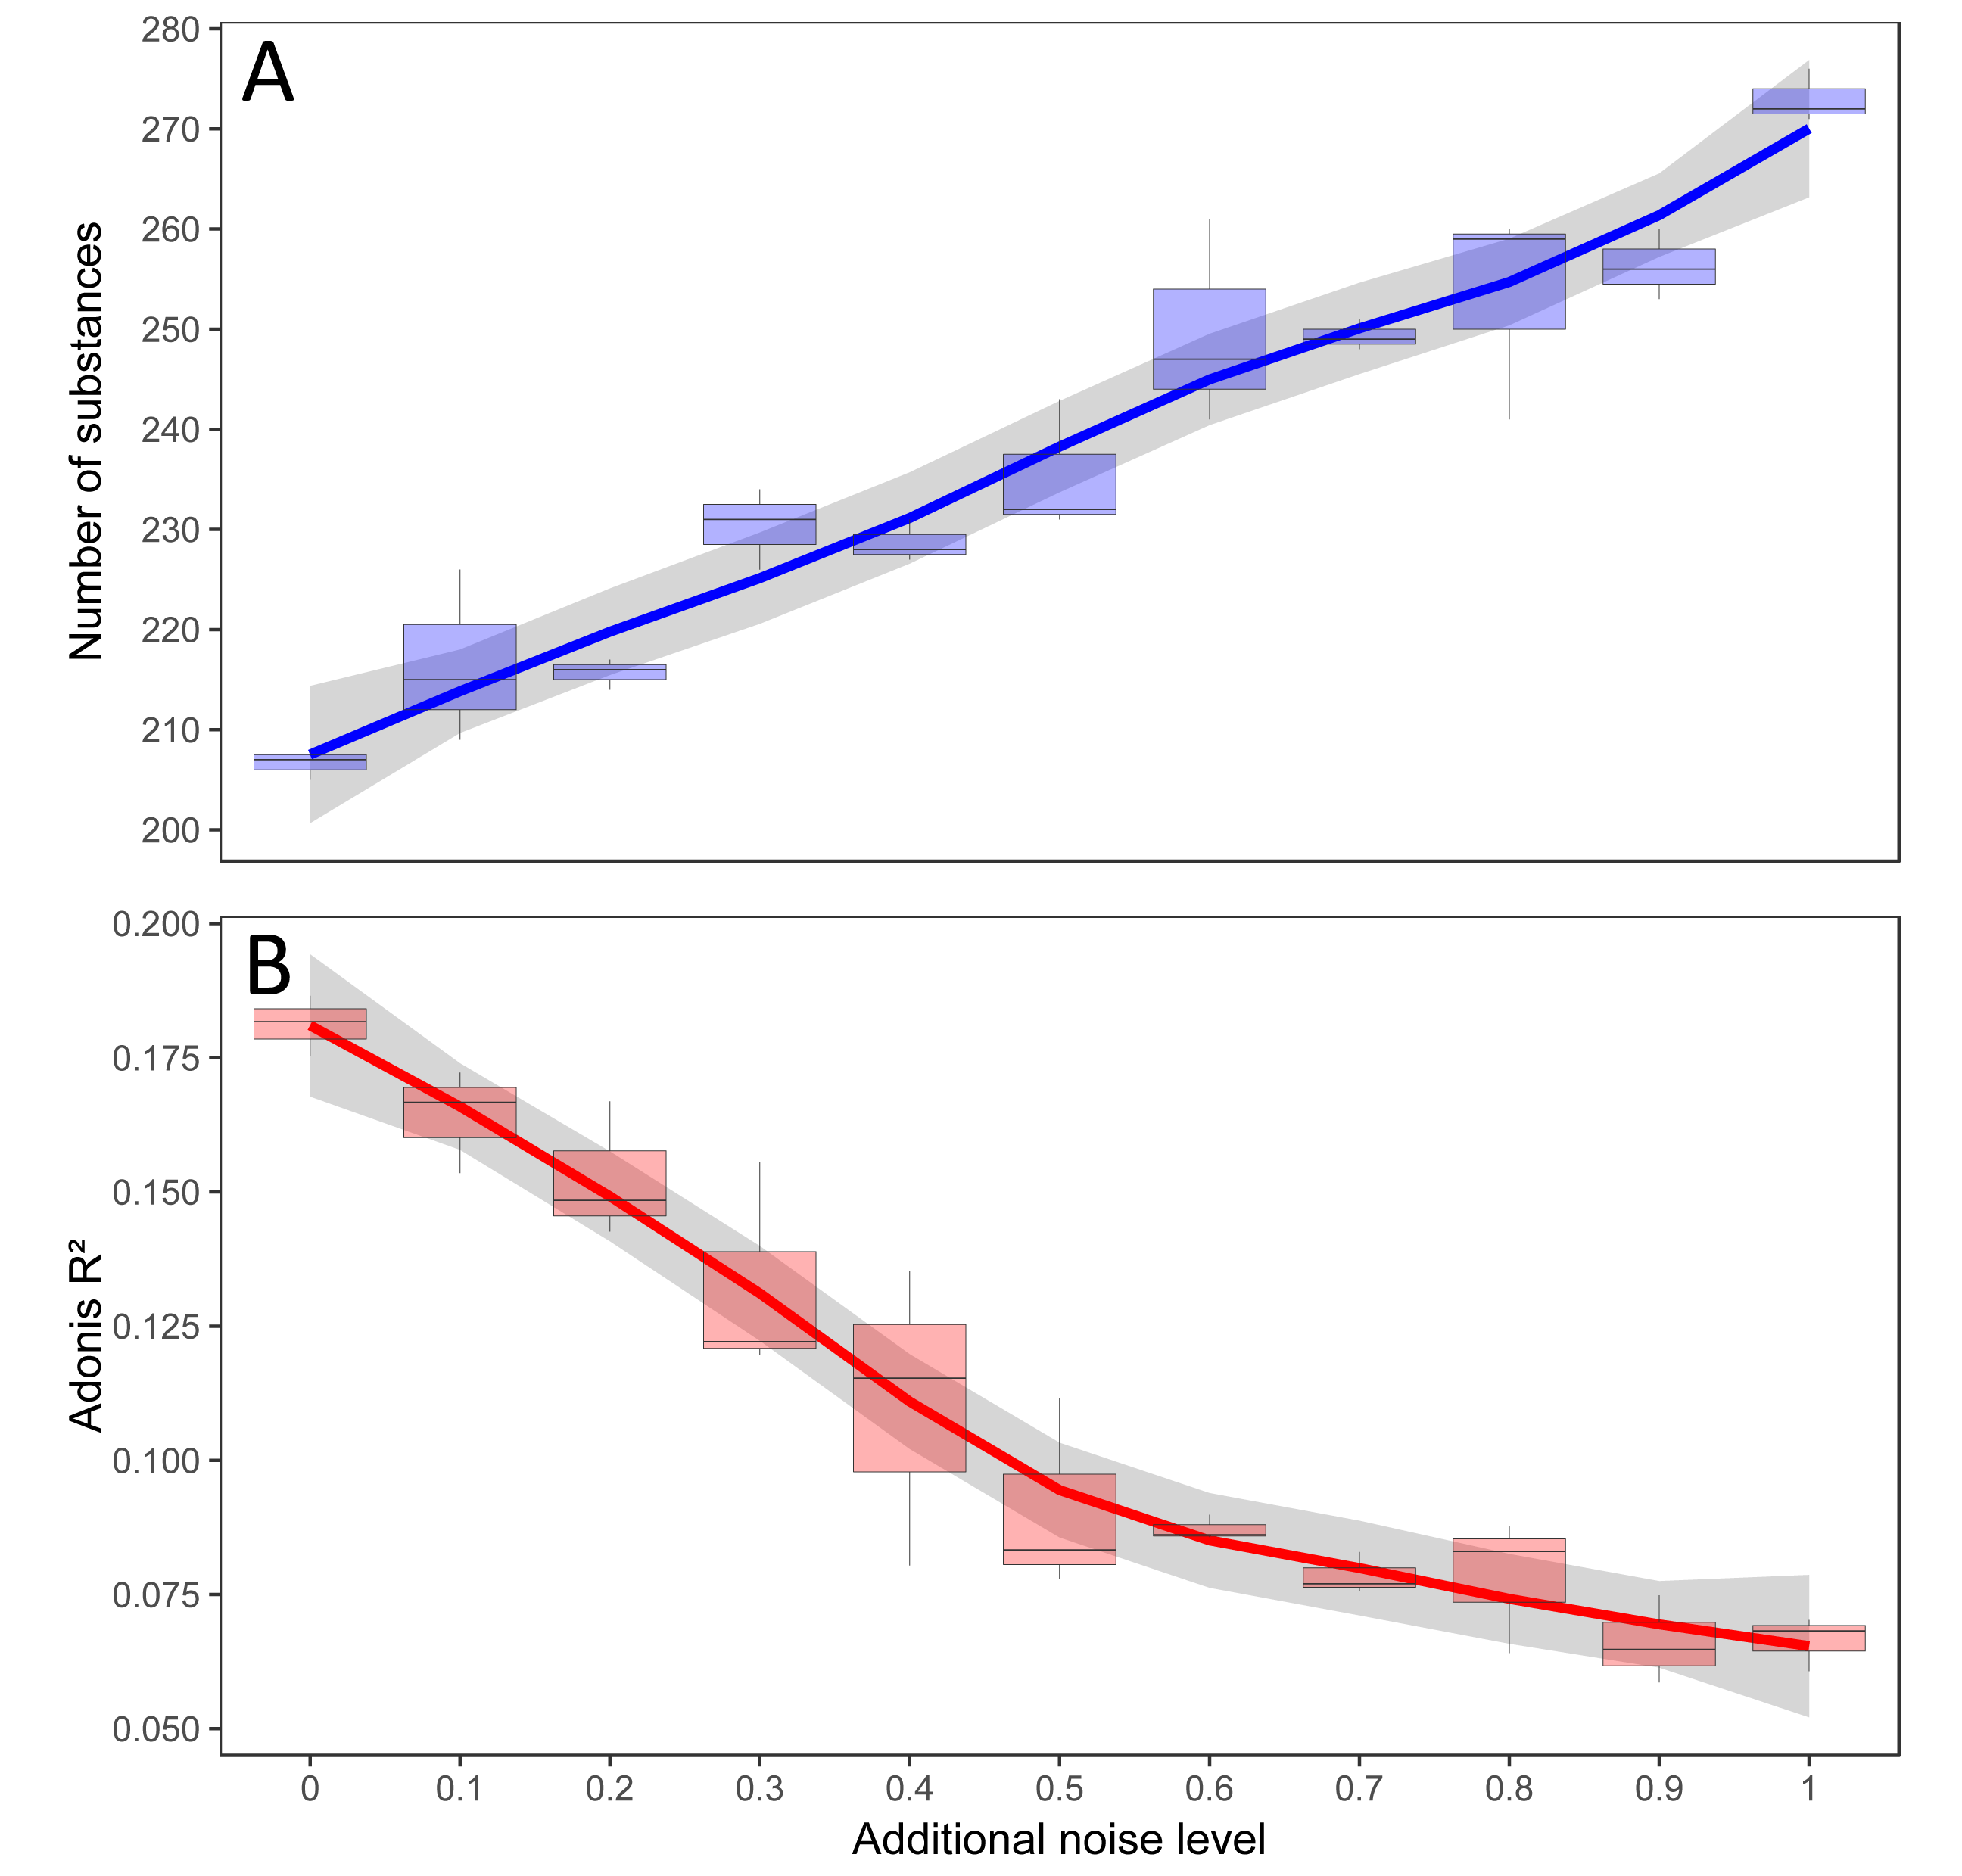
\includegraphics[width=13cm]{figures/adonis}
\caption{Influence of additional noise (random errors) on the total number of scored substances and the strength of the colony effect.}
\label{figure:adonis}
\end{figure}

Introducing errors into the fur seal dataset affected both the total
number of scored substances as well as the strength of the detected
pattern (figure \href{figure:adonis}). The total number of substances
scored gradually increased with increasing error rate (figure
\href{figure:adonis} a) as higher variation in retention times caused
peaks to be split into more than one substance. In parallel, Adonis R2
values fell linearly up to an error rate of 0.5 before levelling off at
around 0.07 (say something about significance, still highly
significant!). This suggests both that the original dataset is clearly
structured and that the results of the alignment procedure within
GCalignR are relatively robust to low to moderate (i.e. \textless{} 0.2)
rates of peak calling error.

\subsection{Validation based on error rates of known
substances}\label{validation-based-on-error-rates-of-known-substances}

To further assess the performance of GCalignR, we calculated alignment
error rates based on three previously published bumblebee datasets
comprising known substances identified using GC-MS
\citep{Dellicour.2013}. The first dataset comprises 24 \emph{Bombus
bimaculatus} individuals characterised for 32 substances (total = 717
retention times). The second comprises 20 \emph{B. ephippiatus}
individuals characterised for 42 substances (total = 782 retention
times) and the third comprises 11 \emph{B. flavifrons} individuals
characterised for 44 substances (total = 457 retention times). We
calculated the error rate as the ratio between incorrectly assigned
retention times and the total number of retention times (equation
\eqref{eq:one}).

\begin{equation}
\label{eq:three}
Error = \left[\frac{N_{missaligned}}{N_{total}}\right] 
\end{equation}

where \emph{N} denotes the number of retention times defined as being
misaligned (i.e.~not assigned to the row that defines the mode of a
given substance). By systematically changing the two parameters
\texttt{max\_diff\_peak2mean} and \texttt{min\_diff\_peak2peak}, we
explored 100 parameter combinations to explore how parameter values
affect the alignment accuracy. All three datasets show generally low
error rates, typically between 3--5\% for most parameter combinations,
although low values of the parameter min\_diff\_peak2peak tend to be
associated with somewhat higher error rates, especially when
max\_diff\_peak2mean is also low (figure \href{figure:parameterspace}).

\begin{figure}[htbp]
\centering
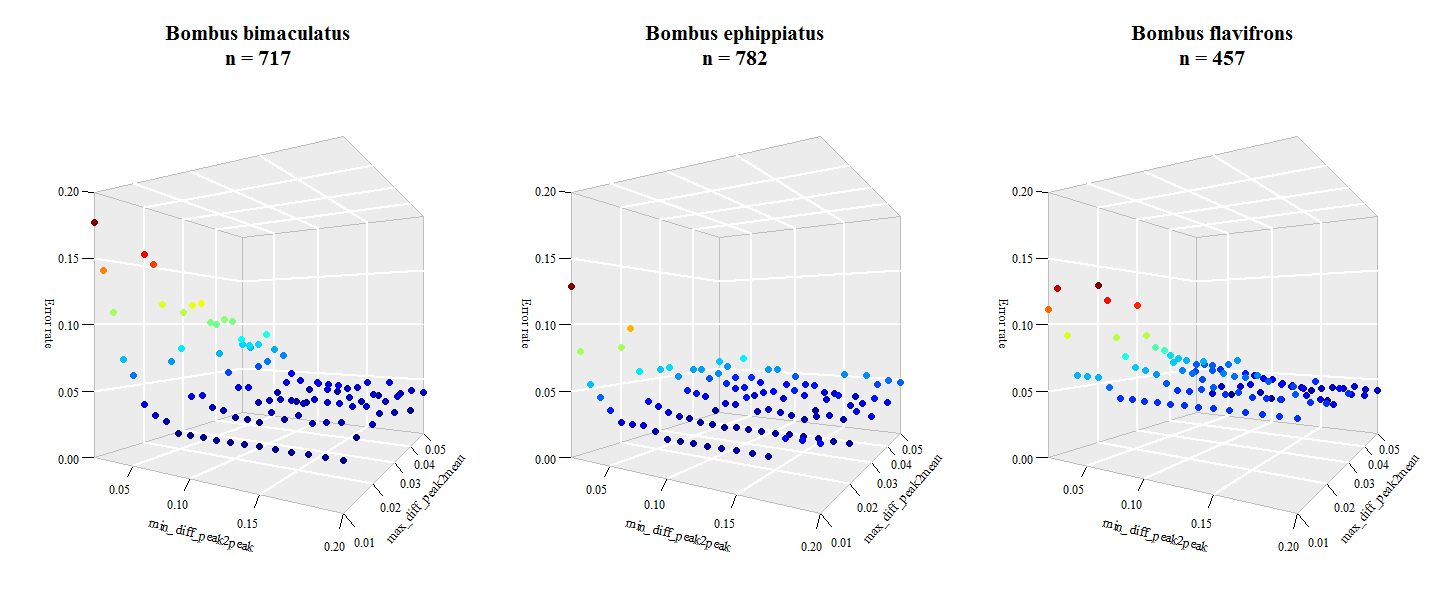
\includegraphics[width=13cm]{figures/parameter_space}
\caption{Effects of alignment parameters on the error rate of three datasets comprising known substances (data of \citet{Dellicour.2013}). Each point shows the error in aligning substances for a combination of max\textunderscore diff\textunderscore peak2mean and min\textunderscore diff\textunderscore peak2peak.}
\label{figure:parameterspace}
\end{figure}

Additionally, we simulated the effect of noise by introducing errors at
random into each of the datasets as described for the fur seal dataset
above. As expected, error rates were initially low for all three species
but increased with progressively increasing levels of noise (figure
\href{figure:noise}). \emph{B. bimaculatus} and \emph{B. flavifrons}
both showed approximately linear responses whereas B. ephippiatus began
to level off when exceeding an additional noise level of around 0.7.
This probably reflects the fact that chemical diversity is lower in
\emph{B. ephippiatus} (stats).

\begin{figure}[htbp]
\centering
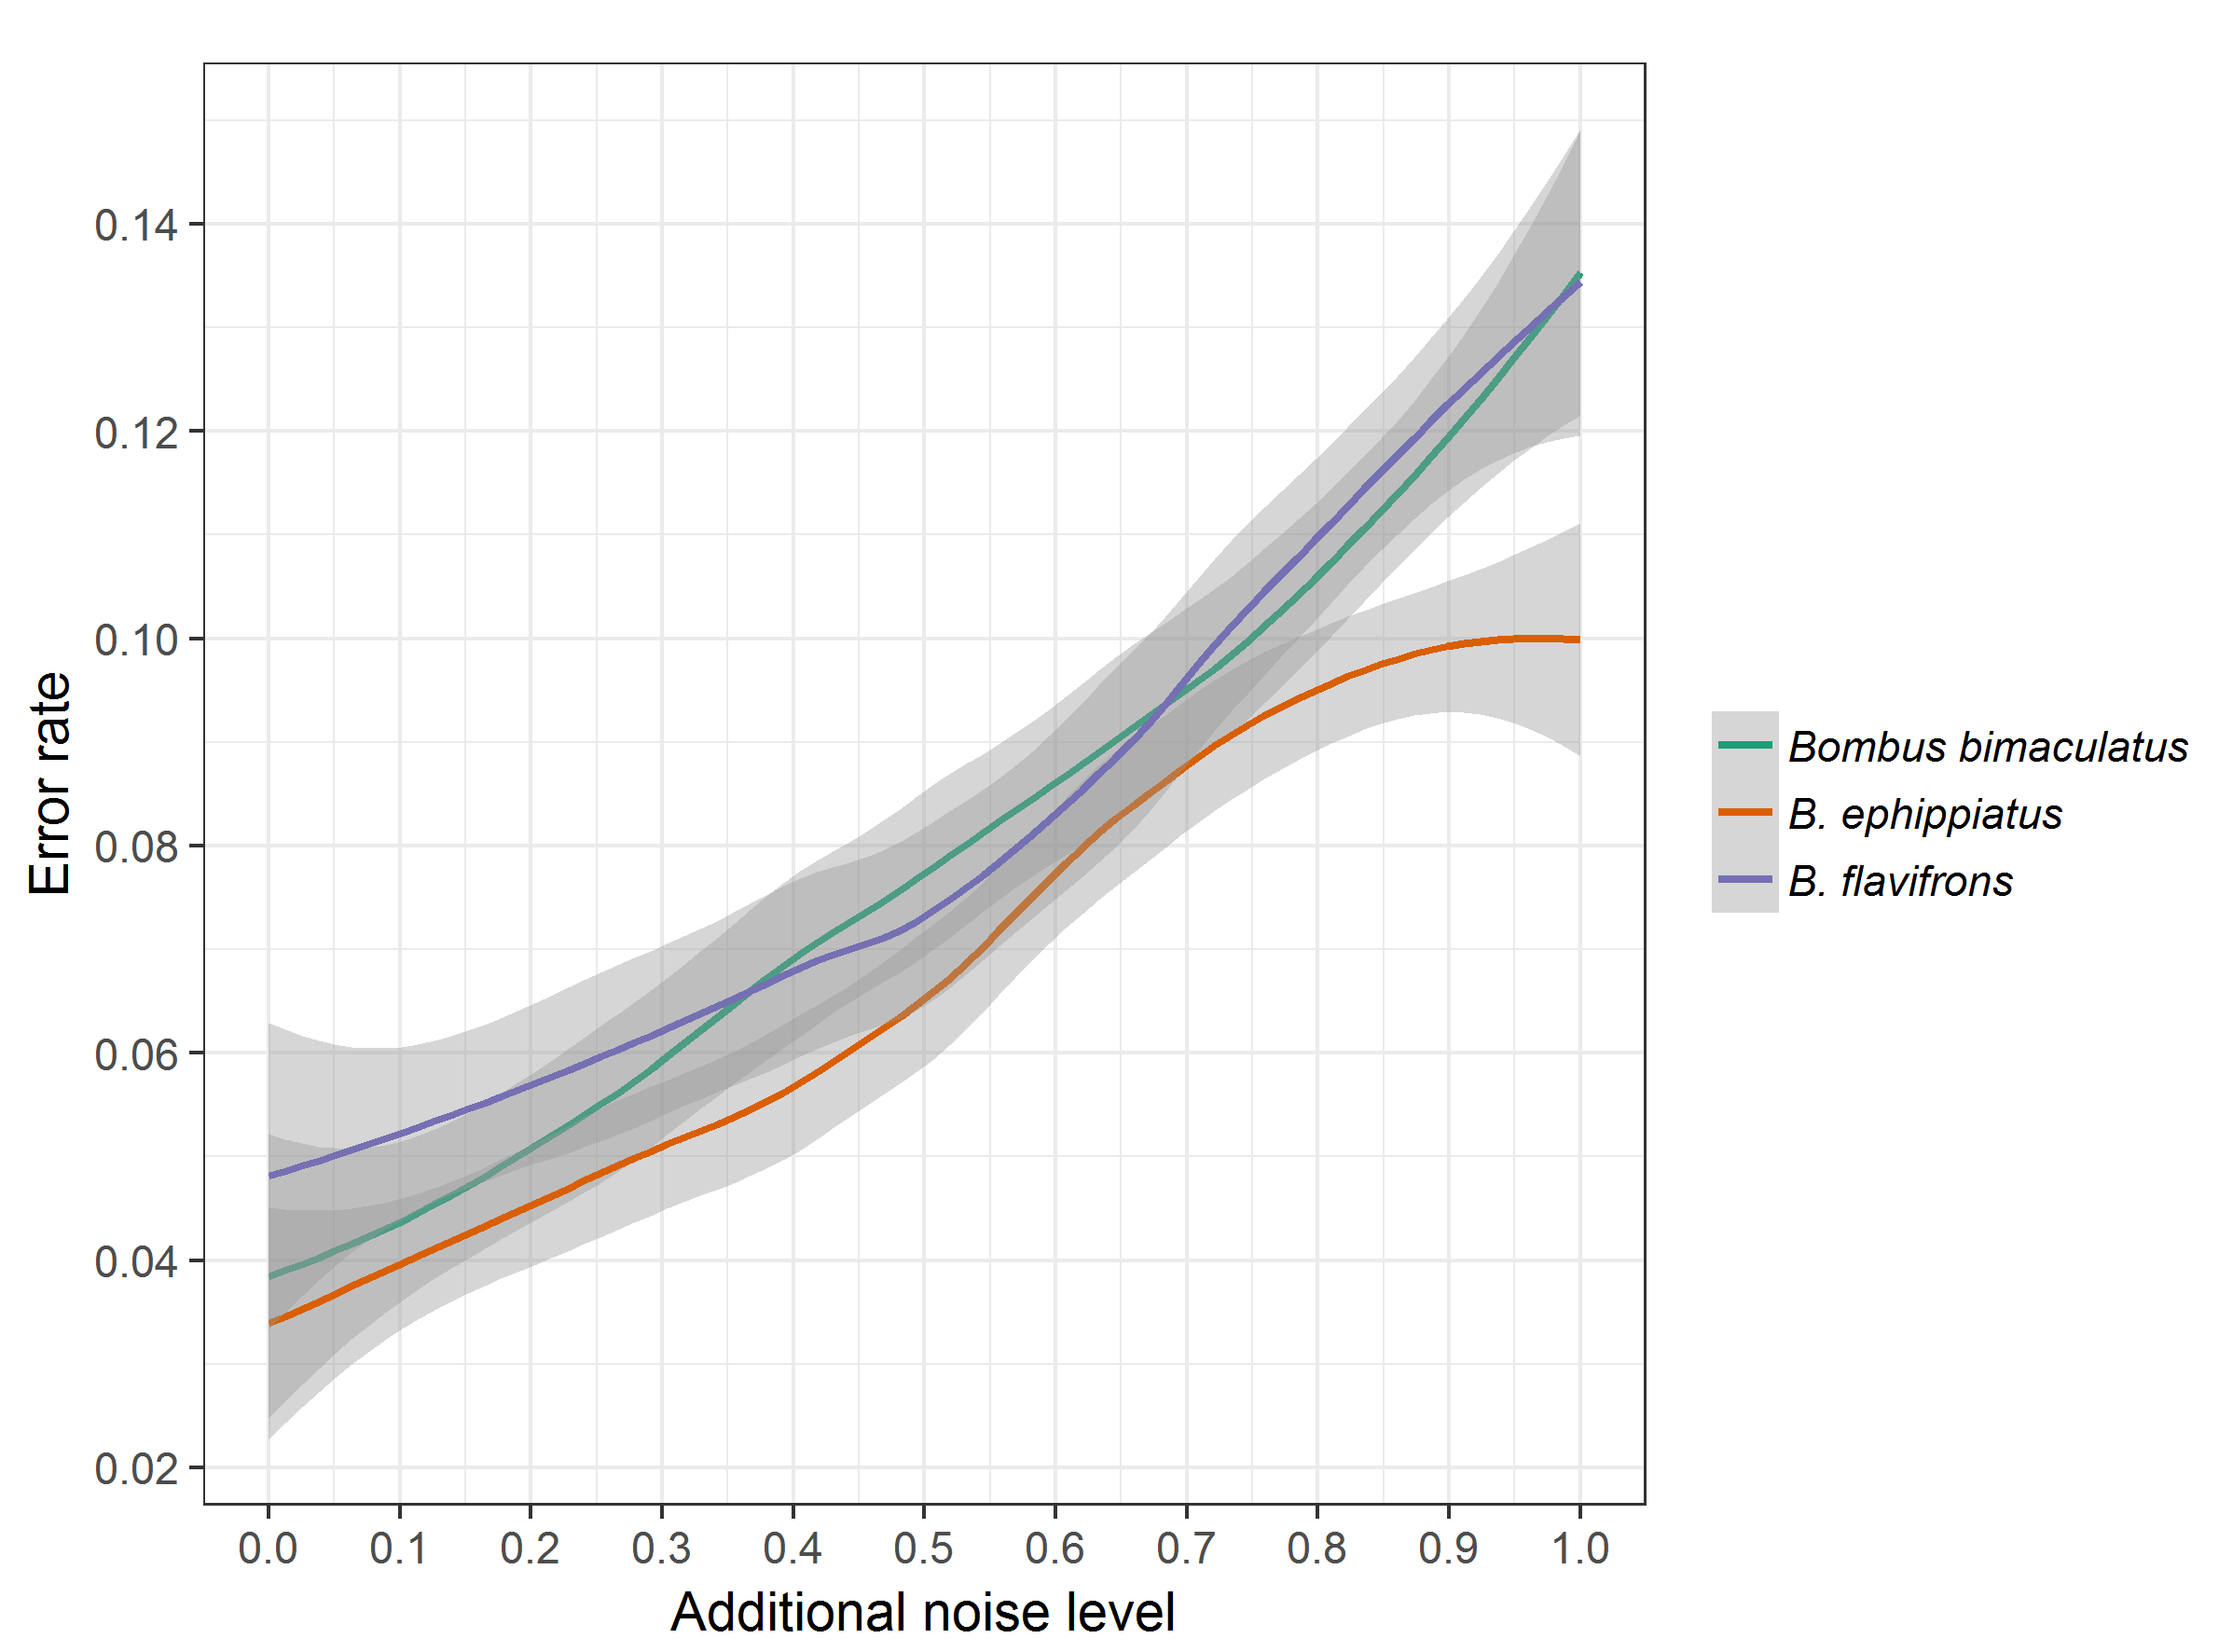
\includegraphics[width=13cm]{figures/noise_simulation}
\caption{Additional noise in peak retention times increases the error rate substantially. Therefore, optimal alignments require clearly resolved peaks that need to be extracted prior to using \pkg{GCalignR}}
\label{figure:noise}
\end{figure}

\subsection{Final remarks}\label{final-remarks}

\texttt{GcalignR} is primarily intended as a pre-processing tool in the
analysis of complex chemical signatures of animals where overall
patterns of chemical similarity are of interest as opposed to specific
(i.e.~known) chemicals. We have therefore prioritised an objective and
fast alignment procedure that is not claimed to be free of error.
However, error rate calculations suggest that the algorithm performs
well, at least for most parameter combinations, while realistically low
levels of noise appear to have a modest effect on the resulting
alignments. Importantly, \texttt{GCaligner} also implements a suite of
diagnostic plots that allow the user to visualise the influence of
parameter settings on the resulting alignments, allowing fine-tuning of
both the pre-processing and alignment steps (figure
\href{figure:workflow}).

\subsection{Availability}\label{availability}

The current stable version requires at least R 3.2.5 and is available on
\texttt{CRAN}.

\begin{Schunk}
\begin{Sinput}
install.packages("GCalignR")
\end{Sinput}
\end{Schunk}

We aim to extend the functionalities of \pkg{GCalignR} in future and the
developmental version can be downloaded from GitHub within R using
\href{https://cran.r-project.org/web/packages/devtools/index.html}{\CRANpkg{devtools}}
\citep{Wickham.2016}.

\begin{Schunk}
\begin{Sinput}
devtools::install_github("mastoffel/GCalignR", build_vignettes = TRUE)
\end{Sinput}
\end{Schunk}

\subsection{Data accessibility}\label{data-accessibility}

The code used to generate these results and accompanying documentation
are provided in a single PDF file written in Rmarkdown (S1) along with
the necessary data (S2). The raw fur seal chemical dataset is included
in this R package and the bumblebee datasets \citep{Dellicour.2013} can
be downloaded here as a
\href{http://onlinelibrary.wiley.com/store/10.1002/jssc.201300388/asset/supinfo/jssc3437-sup-0001-TableS1.zip?v=1&s=57d5d58273d1d4207e70c72cecd5bba4b1fe95a1}{zip-archieve}.

\bibliography{ottensmann-stoffel-hoffman}

\address{%
Meinolf Ottensmann\\
Department of Animal Behaviour\\
Bielefeld University\\ Morgenbreede 45\\ 33615 Bielefeld\\
}
\href{mailto:meinolf.ottensmann@web.de}{\nolinkurl{meinolf.ottensmann@web.de}}

\address{%
Martin A. Stoffel\\
Department of Animal Behaviour\\
Bielefeld University\\ Morgenbreede 45\\ 33615 Bielefeld\\
}
\href{mailto:Martin.Adam.Stoffel@gmail.com}{\nolinkurl{Martin.Adam.Stoffel@gmail.com}}

\address{%
Joseph I. Hoffman\\
Department of Animal Behaviour\\
Bielefeld University\\ Morgenbreede 45\\ 33615 Bielefeld\\
}
\href{mailto:j_i_hoffman@hotmail.com}{\nolinkurl{j\_i\_hoffman@hotmail.com}}

